\documentclass[border=5pt]{standalone}

\usepackage[utf8]{inputenc}
\usepackage{garamondx}

\usepackage[x11names]{xcolor}
\usepackage{tikz}
\usetikzlibrary{shapes.geometric, arrows, positioning}

\definecolor{darkolivegreen}{rgb}{0.33, 0.42, 0.18}
\definecolor{darkbyzantium}{rgb}{0.36, 0.22, 0.33}
\definecolor{darkelectricblue}{rgb}{0.33, 0.41, 0.47}

\tikzstyle{background}=[rectangle, rounded corners, minimum width=7em, minimum height=2em, text centered, draw=black, fill=darkolivegreen!30, text width=7em]
\tikzstyle{process} = [rectangle, rounded corners, minimum width=7em, minimum height=2em, text centered, draw=black, fill=darkbyzantium!30, text width=7em]
\tikzstyle{psych}=[rectangle, rounded corners, minimum width=10em, minimum height=2em, text centered, draw=black, fill=darkelectricblue!30, text width=7em]
\tikzstyle{arrow}=[very thick, ->,>=latex]
\tikzstyle{arrow'}=[very thick, <->, >=latex]

\begin{document}
	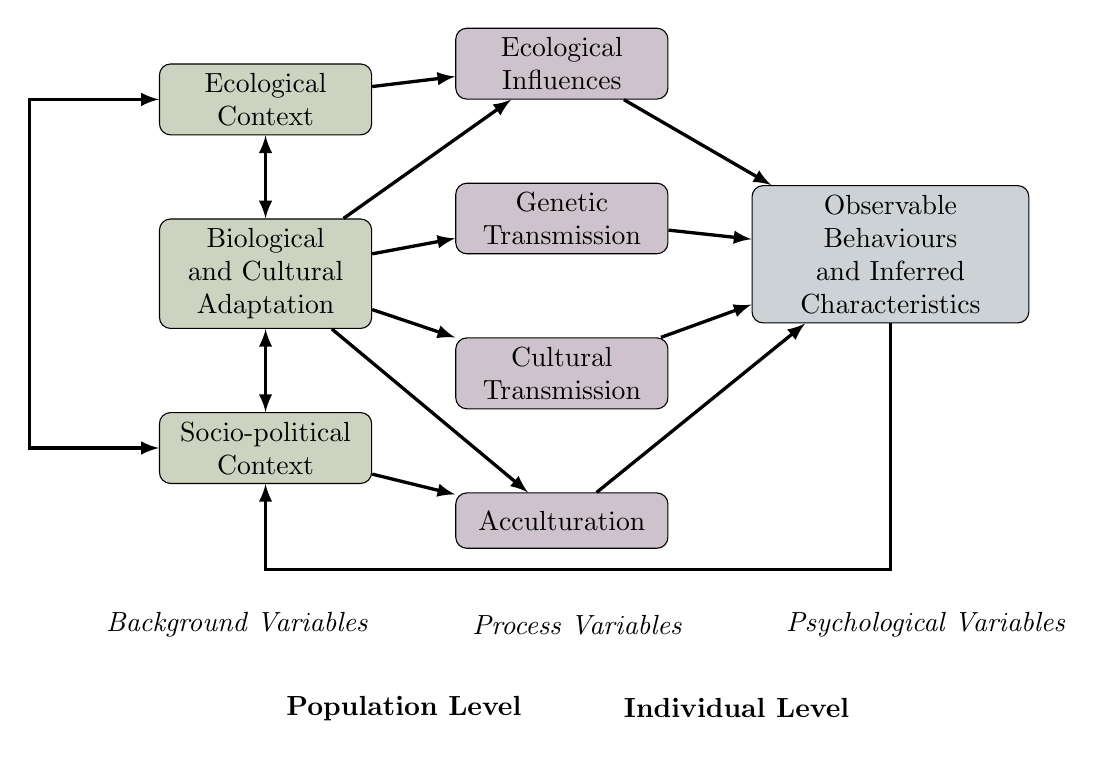
\begin{tikzpicture}[node distance=3em]
		\node(background1)[background]{Ecological Context};
		\node (background2) [background, below=of background1]{Biological and Cultural Adaptation};
		\node(background3)[background, below=of background2]{Socio-political Context};
		
		\node(process1)[process, right=of background1, yshift=3ex]{Ecological Influences};
		\node(process2)[process, right=of background2, below=of process1]{Genetic Transmission};
		\node(process3)[process, right=of background3, below=of process2]{Cultural Transmission};
		\node(process4)[process, right=of background3, below=of process3]{Acculturation};
		
		\node(psych1)[psych, right=of process2, yshift=-3ex]{Observable Behaviours and Inferred Characteristics};
		
		\draw[arrow](background1)--(process1);
		\draw[arrow](background2)--(process1);
		\draw[arrow](background2)--(process2);
		\draw[arrow](background2)--(process3);
		\draw[arrow](background2)--(process4);
		\draw[arrow](background3)--(process4);
		\draw[arrow'](background1)--(background2);
		\draw[arrow'](background2)--(background3);
		\draw[arrow](process1)--(psych1);
		\draw[arrow](process2)--(psych1);
		\draw[arrow](process3)--(psych1);
		\draw[arrow](process4)--(psych1);
		\draw [arrow] (psych1) -- ++(0,-2) -- ++(0,-2) -| (background3);
		\draw[arrow'](background1)-- ++(-1.5,0) -| ++(-1.5,0) |-(background3);
		
		\node[below=of background3, yshift=-10ex, xshift=5em](poplevel){\textbf{Population Level}};
		\node[right=of poplevel](indivlevel){\textbf{Individual Level}};
		\node[below=of background3, yshift=-3ex, xshift=-1em](background){\emph{Background Variables}};
		\node[right=of background](process){\emph{Process Variables}};
		\node[right=of process](psych){\emph{Psychological Variables}};
	\end{tikzpicture}
\end{document}
